% !TeX root = ../index.tex
\documentclass[../index.tex]{subfiles}

\begin{document}
    \section{Wykład}
        \subsection{Układy podwójne}
            Często występującym układem gwiazd są układy podwójne. W zależności od odległości od siebie ewolucja tych gwiazd może być identyczna jak gwiazd samotnych jak i silnie zaburzona obecnością sąsiada. Niech \(M_1\), \(M_2\) to masy gwiazd, które rotują z prędkością kątową \(\omega\) wokół środka masy znajdującego się w odległości odpowiednio \(r_1\) i \(r_2\). Na punkt materialny \(m\) działają sił \(F_g\) (grawitacji) i \(F_c\) (siła odśrodkowa). Związane z tymi siłami potencjały oznaczone są odpowiednio \(\phi_g\) i \(\phi_c\), a ich suma, zwana \textbf{potencjałem efektywnym} – \(\phi\). Punkt \(m\) znajduje się w odległościach \(s_1\) i \(s_2\) od gwiazd:
            \begin{align}
                F_c &=  m\omega^2 r\\
                \phi_c &=  - \frac{1}{2}m\omega^2  r^2 \\
                F_g &=  Gm\autosquare{\frac{M_1}{s_1^2 } +\frac{M_2}{s_2^2 } }\\
                \phi_g &= - G \autoround{\frac{M_1m}{s_1} + \frac{M_2m}{s_2}  } \\
                \phi &=  - G\autoround{\frac{M_1m}{s_1} +\frac{M_2m}{s_2}  } - \frac{1}{2}m\omega^2 r^2 
            \end{align}
            Poniżej obraz linii ewkipotencjalnych przykładowego układu podwójnego. 
            \begin{center}
                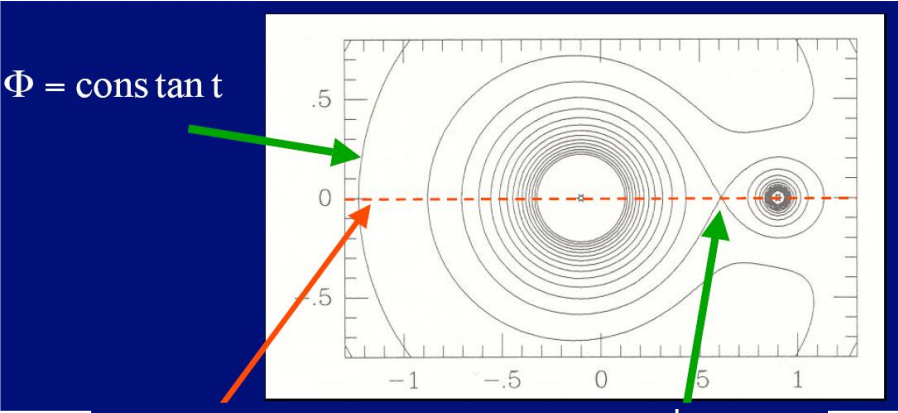
\includegraphics[width=13cm]{images/ukladPodwojnyPotencjal.png}
            \end{center}
            Zielona, niepodpisana strzałka wskazuje na punktu \(L_1\) – punkt Lagrange 1. Jest to punkt lokalnego maksimum potencjału (jest ich więcej). Powierzchnie ekwipotencjalne przecinające się w \(L_1\) noszą nazwę \textbf{krytycznych powierzchni Roche'a}. Wszystkie punkty materialne znajdujące się wewnątrz tych powierzchni są związane z jedną z gwiazd, natomiast punkty na zewnątrz są związane z układem jako z całością. Jeśli jedna z gwiazd będzie wystawać poza krytyczne powierzchnie Roche'a, to wówczas zacznie tracić swoją materię na rzecz sąsiada. Ze względu na to zjawisko układy podwójne dzieli się na:
            \begin{itemize}
                \item układy rozdzielone
                \begin{center}
                    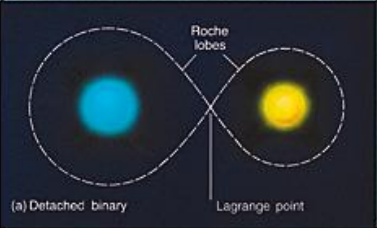
\includegraphics[width=10cm]{images/ukladPodwojnyRozdzielone.png}
                \end{center}
                \item układy półrozdzielone
                \begin{center}
                    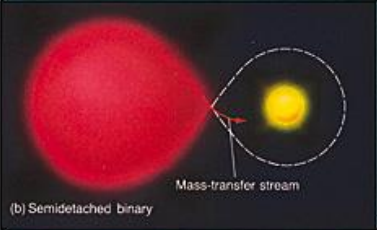
\includegraphics[width=10cm]{images/ukladPodwojnyPolrozdzielone.png}
                \end{center}
                \item układy kontaktowe
                \begin{center}
                    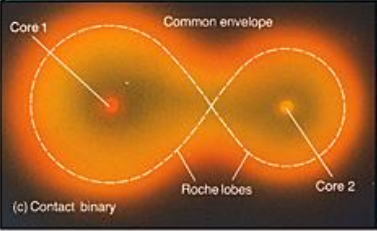
\includegraphics[width=10cm]{images/ukladPodwojnyKontaktowe.png}
                \end{center}
            \end{itemize}
            Należy pamiętać, że w wyniku ewolucji gwiazd ich masa i rozmiar zmieniają sie, więc układy pierwotnie rozdzielone mogą stać się kontaktowe i vice versa (np. poprzez odrzucenie otoczki). Przykładem ewolucji układu podwójnego, w którym doszło do zmiany jego typu jest \textbf{paradoks Algola}. Obserwując ten układ można zauważyć układ dwóch gwiazd: B – mniej masywnego olbrzyma i A – bardziej masywnego karła. Wiadomo, że mniej masywne gwiazdy ewoluują wolniej, więc jak powstał taki układ? Składnik B był dawniej bardziej masywny i szybciej opuścił ciąg główny, tym samym zaczął oddawać część swojej masy składnikowi A. Proces ten wciąż trwa. Potrafimy zidentyfikować w widmie układu \textbf{gorącą plamę}– punkt, w którym z gwiazdy-dawcy wypływa materia (punkt \(L_1\)).
            \begin{center}
                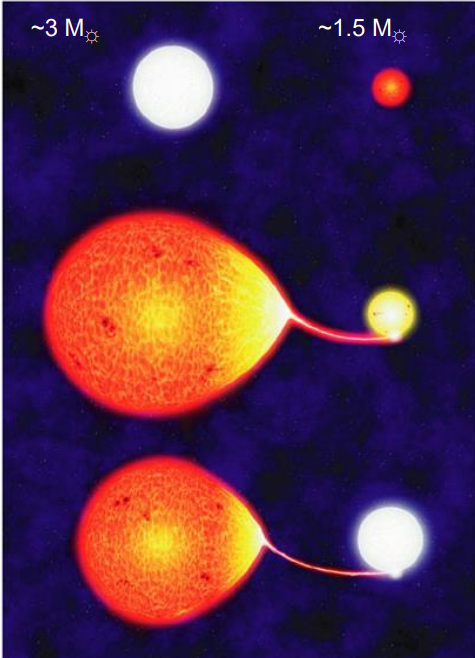
\includegraphics[width=6cm]{images/algol.png}
            \end{center}
            Innym przypadkiem jest sytuacja, gdy gwiazda-biorca jest na tyle mała, że materia wypływająca z gwiazdy-dawcy nie trafia w nią bezpośrednio, a formuje wokół niej dysk z materii – \textbf{dysk akrecyjny}. Zanim materia z dysku spadnie na gwiazdę, musi wytracić sporą część momentu pędu. W wyniku tarcia pomiędzy poszczególnymi warstwami dysku (\textbf{lepkość}), kształtuje się, w raz odległością od biorcy, rozkład momentu pędu i temperatury. Im bliżej gwiazdy tym moment pędu mniejszy, a temperatura większa. O dyskach mówi się czasami, że są to płaskie gwiazdy.
            \begin{center}
                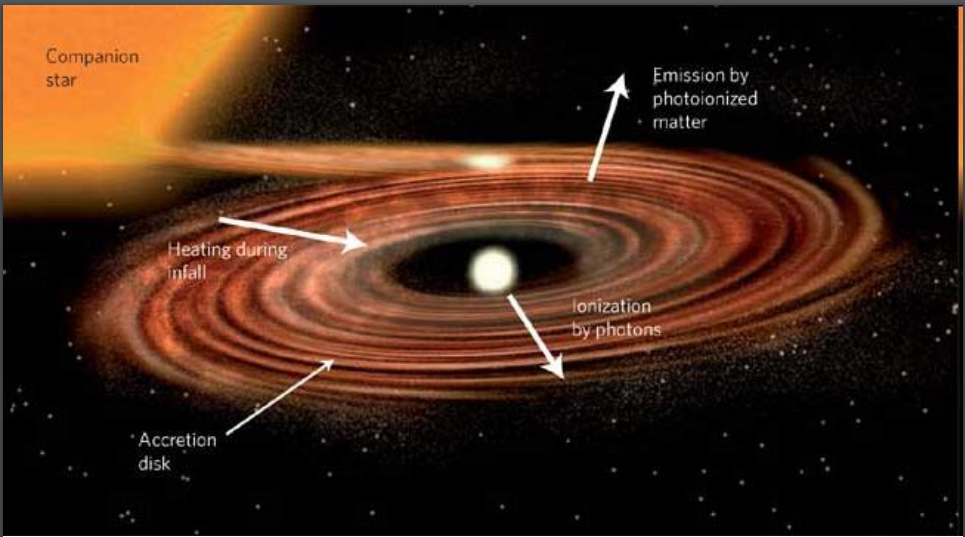
\includegraphics[width=13cm]{images/accretionDisk.png}
            \end{center}
            W przypadku gdy gwiazdą biorcą jest biały karzeł, gwiazda neutronowa lub czarna dziura, dysk emituje spore ilości energii (grawitacyjnej) w formie promieniowania elektromagnetycznego. Moc tego promieniowania wyznaczana jest według wzoru:
            \begin{equation}
                L \approx \frac{GM_a}{R_a} \frac{\dd M}{\dd t}
            \end{equation}
            gdzie \(M_a\) i \(R_a\) to masa i promień biorcy, a \(\frac{\dd M}{\dd t} \) to tempo akrecji. \textbf{Wydajność akrecji} to stosunek \(L\) do ilości energii, która wydzieliła by się w wyniku anihilacji materii akreującej:
            \begin{equation}
                \eta = \frac{L}{\frac{\dd M}{\dd t} c^2  } = \frac{G}{c^2 }\frac{M_a}{R_a} 
            \end{equation}
            Przykładowe wartości \(\eta\): biały karzeł – \(10^{ - 4}\), gwiazda neutronowa – \(0.2\) i czarna dziura – \(0.5\). W przypadku białych karłów większość energii wypromieniowana jest w świetle widzialnym, a w przypadku gwiazd neutronowych i czarnych dziur w paśmie promieniowania X. \\
            Częstym zjawiskiem w układach podwójnych z białymi karłami są \textbf{gwiazdy nowe} i \textbf{nowe karłowate}(zaliczane do \textbf{gwiazd kataklizmycznych}). W wyniku opadania na powierzchnie białego karła materii z drugiej gwiazdy (z dysku akrecyjnego) inicjowane są tam reakcje termojądrowe. Mają one postać wybuchu – obserwuje się gwałtowny i silny wzrost jasności – gwiazda nowa. Po krótkim czasie karzeł oczyszcza się z wodoru i jego jasność wraca do wcześniejszego poziomu. Akrecja nadal trwa więc za jakiś proces się powtórzy. Nowy karłowate także są okresowy pojaśnieniami, lecz w ich przypadku odpowiada za to dysk akrecyjny. Pod wpływem akumulacji materii na dysku rośnie temperatura w całym jego obrębie. Proces ten przyspiesza akrecje na biała karła, a to zmniejsza ilość materii oraz temperature itd. Pojaśnienie jest związane z fazą rozgrzanego dysku.\\
            Akrecja może zachodzić nieco inaczej, gdy gwiazda-biorca charakteryzuje sie wyjątkowo silnym polem magnetycznym. Wówczas akrecja odbywać się bedzie wzdłuż linii pola, a układ nazywany jest \textbf{polarem}.
            \begin{center}
                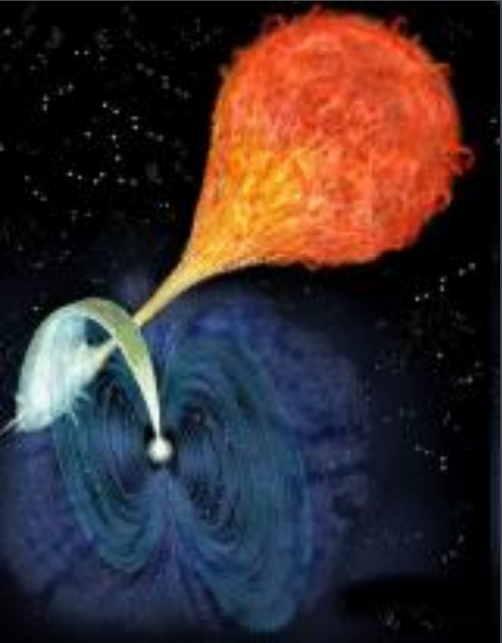
\includegraphics[width=7cm]{images/polar.png}
            \end{center}
            Gdy biały karzeł, w wyniku przybierania na masie, przekroczy granicę Chandrasekhara, wówczas zamiast kolapsu do gwiazdy neutronowej, gwałtownie rosnące procesy termojądrowe doprowadzają do rozerwania gwiazdy. Takie zjawisko nazywa sie \textbf{supernową typu Ia}. W wybuchu uczestniczy zwykle podobna ilość materii, stąd jasność tego typu supernowych jest bardzo zbliżona i można je używać jako \textbf{świece standardowe} – do wyznaczania odległości w przestrzeni kosmicznej.\\ 
            W przypadku akrecji materii na gwiazdę neutronową lub czarną dziurę, wewnętrzna część dysku rozgrzewa się do milionowych temperatur i świeci w zakresie promieniowania X. W tym przypadku wyróżnia się dwa rodzaju układów ze względu na masę gwiazdy-dawcy:
            \begin{itemize}
                \item \textbf{LMXB} – gdy masa dawcy jest porównywalna z masą słońca przepływ materii odbywa się w formie strugi wypływającej z \(L_1\). Inaczej niż w układach z białymi karłami gwiazda-dawca jest ogrzewany przez gorący dysk oraz z biegunów gwiazdy-biorcy wychodzą skolimowane wiązki materii zwane \textbf{dżetami}.
                \item \textbf{HMXB} – gdy masa dawcy jest znacznie większa, zasilanie biorcy umożliwia obfity wiatr gwiazdowy.
            \end{itemize}
            W przypadku tych układów można też wyróżnić odpowiedniki nowych (\textbf{nowe rentgenowskie}) i nowych karłowatych (\textbf{burstery}). W obu przypadkach wybuchy są bardziej dynamiczne niż ich białokarłowych odpowiednikach. Jedyną możliwością odróżnienia tego czy w centrum znajduje się gwiazda neutronowa czy czarna dziura jest pomiar masy.
        \subsection{Gwiazdy pulsujące}
            \textbf{Gwiazdy pulsujące} to takie, których jasność ulega cyklicznym zmianą. Przyczyn zmienności gwiazd jest bardzo wiele. Pierwszą odkrytą była \(\delta\)–Cephei, od której wzięła się nazwa podkategorii gwiazd zmiennych – \textbf{cefeidy}. W przypadku tej gwiazdy za zmianę jasności odpowiedzialne są naprzemienne procesy rozdymania się i kurczenia, które skutkują względnymi zmianami jasności do 15\%. Taka sama jest przyczyna zmiany jasności wszystkich gwiazd pulsujących, jednak wielkość zmian może być zarówno bardzo wyraźna jak i subtelna. Pulsacje w gwiazdach mogą być bardzo złożone, w szczególności w tym samym czasie niektóre fragmenty gwiazdy mogą się kurczyć, a inne rozdymać. Możliwe jest też pulsowanie \textbf{nieradialne} czyli takie, w którym w tej samej odległości od środka dopuszczalny jest ruch zarówno do środka, jak i na zewnątrz. Badanie tych wszystkich subtelności zajmuje się \textbf{asterosejsmologia}.\\
            Gwiazdy pulsacyjne zajmują konkretny obszar na wykresie H-R nazywany \textbf{pasem niestabilności pulsacyjnej gwiazd}, a sama podatność na pulsowanie wykazywana jest tylko na pewnych etapach ewolucji. Efekt pulsowania bierze się z faktu, że w odpowiednich warunkach duża ilość promieniowania może być pochłania w celu jonizacji metali (wiąże się to ze wzrostem \(\kappa\) – współczynnika absorbcji promieniowania), helu i wodoru. Gdy gwiazda się kurczy właśnie w zjonizowanych pierwiastkach magazynowana jest energia, która zostanie użyta w etapie rozkurczania (do pokonywania siły grawitacji).\\
            Gwiazdy pulsujące, a w szczególności cefeidy, także pełnią rolę świec standardowych. Znana jest zależność między okresem pulsacji cefeidy i jej jasnością a odległością do niej (trzeba brać pod uwagę skład chemiczny gwiazdy).
\end{document}